\documentclass{../../oss-apphys-exam}
\newcounter{lastmc}

\begin{document}
%\genheader

\gentitle{6}{CIRCULAR MOTION}

%\genmultidirections
%\gengravity

\raggedcolumns
\begin{multicols*}{2}
  \begin{questions}
    \question A girl stands on a rotating merry-go-round without holding on to
    a rail. The force that keeps her moving in a circle is the
    \begin{choices}
      \choice frictional force on the girl directed away from the center of the
      merry-go-round
      \choice frictional force on the girl directed toward the center of the
      merry-go-round
      \choice normal force on the girl directed away from the center of the
      merry-go-round
      \choice normal force on the girl directed toward the center of the
      merry-go-round
      \choice weight of the girl
    \end{choices}
    \vspace{.7in}
    
    % This problem needs some fixing. None of the answers are correct
%    \question A \SI{.5}{\kilo\gram} ball on the end of a \SI{.5}{\metre} long
%    string is swung in a horizontal circle. What would the speed of the ball 
%    have tobe for the tension in the string to be \SI{9.}{\newton}?
%    \begin{choices}
%    \choices\SI1{\metre\per\second}
%    \choices\SI3{\metre\per\second}
%    \choices\SI6{\metre\per\second}
%    \choices\SI9{\metre\per\second}
%    \choices\SI{12}{\metre\per\second}
%    \end{choices}

%    \uplevel{
%      \begin{center}
%        \begin{tikzpicture}
%          \fill circle (.08);
%          \fill (0,1.2) circle (.06);
%          \draw[thick,dashed] ellipse (3 and 1.2);
%          \draw[thick,dashed] (0,1.7)--(0,-1.5);
%          \draw[thick] (-3,0)--(0,1.2);
%          \draw[thick,fill=white] (-3,0) circle (.12) node[left]{$m$};
%          \draw[<->] (0,1.5)--(-3,1.5) node[midway,above]{$R$};
%          \draw[dashed] (0,1.2)--(-2,1.2);
%          \draw[->] (-1.5,1.2) arc (180:202:1.5) node[midway,left]{$\theta$};
%          \draw[vectors,rotate around={20:(-3,0)}] (-3,0)--(-3,-1)
%          node[below]{$v$};
%        \end{tikzpicture}
%      \end{center}
%
%      \textbf{Questions \ref{ball1}--\ref{ball2}}:
%      A ball of mass $m$ and weight $W$ on the end of a string is swung in a
%      horizontal circle of radius $R$ with a speed $v$. The string makes an
%      angle $\theta$ below the horizontal, as shown. The magnitude of the
%      tension in the string is $T$.
%    }
%
%  \question Which of the following diagrams best shows the forces acting on the
%    ball as it moves in a circle? 
%    \begin{choices}
%      \choice
%      \begin{tikzpicture}[vectors]
%        \fill circle (.05);
%        \draw (0,0)--(0,-1) node[right]{$W$};
%        \draw (0,0)--(1.3,0) node[right]{$F_c$};
%        \draw[rotate=30] (0,0)--(1.5,0) node[right]{$T$};
%      \end{tikzpicture}
%      
%      \choice
%      \begin{tikzpicture}[vectors]
%        \fill circle (.05);
%        \draw (0,0)--(0,-1) node[right]{$W$};
%        \draw (0,0)--(1.5,0) node[right]{$T$};
%      \end{tikzpicture}
%      
%      \choice
%      \begin{tikzpicture}[vetors]
%        \fill circle (.05);
%        \draw (0,0)--(0,-1) node[right]{$W$};
%        \draw[rotate=30] (0,0)--(1.5,0) node[right]{$T$};
%      \end{tikzpicture}
%
%      \choice
%      \begin{tikzpicture}[vectors]
%        \fill circle (.05);
%        \draw (0,0)--(0,-1) node[right]{$W$};
%        \draw (0,0)--(1.5,0) node[right]{$F_c$};
%        \draw (0,0)--(0,1) node[right]{$T$};
%      \end{tikzpicture}
%      
%      \choice
%      \begin{tikzpicture}[vectors]
%        \fill circle (.05);
%        \draw (0,0)--(0,-1) node[right]{$W$};
%        \draw[rotate=120] (0,0)--(1.5,0) node[left]{$T$};
%      \end{tikzpicture}
%    \end{choices}
%    \label{ball1}
%    
%    \question In terms of $m$, $R$, $v$, and $\theta$, the magnitude of the
%    tension $T$ is
%    \begin{choices}
%      \choice $\dfrac{mv^2}R$
%      \choice $\dfrac{mv^2}{R\sin\theta}$
%      \choice $\dfrac{mv^2}{R\cos\theta}$
%      \choice $\dfrac{mv}{R\sin\theta}$
%      \choice $mv R\sin\theta$
%    \end{choices}
%    \label{ball2}
    
    \question A ball of mass $m$ is swung in a vertical circle of radius $R$.
    The speed of the ball at the bottom of the circle is $v$. The tension in
    the string at the bottom of the circle is
    \begin{choices}
      \choice $mg$
      \choice $mg+\dfrac{mv^2}R$
      \choice $mg-\dfrac{mv^2}R$
      \choice $\dfrac{mv^2}R$
      \choice 0
    \end{choices}
    \vspace{.3in}
    
    \question A car of mass $m$ drives on a flat circular track of radius $R$.
    To maintain a constant speed $v$ on the track, the coefficient of
    friction $\mu$ between the tires and the road must be
    \begin{choices}
      \choice $mg$
      \choice $mg+\dfrac{mv^2}R$
      \choice $mg-\dfrac{mv^2}R$
      \choice $\dfrac{v^2}{gR}$
      \choice $\sqrt{\dfrac{v^2}{gR}}$
    \end{choices}
    \columnbreak
    
    \question An airplane traveling at \SI{300}{\metre\per\second} banks its
    wings to enter into a horizontal circular turn. The circular path has a
    radius of \SI{2.7}{\kilo\metre}. Which of these values \emph{best}
    represents the angle of the wings relative to the horizontal if the airplane
    experiences no change in altitude during the turn? Assume that the wings
    are completely horizontal during level flight.
    \begin{choices}
      \choice\ang{8}
      \choice\ang{16}
      \choice\ang{20}
      \choice\ang{25}
      \correctchoice\ang{74}
    \end{choices}
    
%    \uplevel{
%      \textbf{Questions \ref{rad1}--\ref{rad2}}
%    }
%
%    \question A ball on the end of a string is swung in a circle of radius
%    \SI2{\metre} according to the equation $\theta=4t^2+3t$, where $\theta$ is
%    in radians and $t$ is in seconds. The angular acceleration of the ball is
%    \begin{choices}
%      \choice \SI6{rad\per\second\squared}
%      \choice $4t^2 + 3t$ \si{rad\per\second\squared}
%      \choice $8t +3$ \si{rad\per\second\squared}
%      \choice $\dfrac34 t^3 + 3t^2$ \si{\radian\per\second\squared}
%      \choice \SI8{\radian\per\second\squared}
%    \end{choices}
%    \label{rad1}
%    
%    \question The linear speed $v$ of the ball at $t=\SI3\second$ is
%    \begin{choices}
%      \choice \SI{27}{\metre\per\second}
%      \choice \SI{54}{\metre\per\second}
%      \choice \SI{108}{\metre\per\second}
%      \choice \SI{135}{\metre\per\second}
%      \choice \SI{210}{\metre\per\second}
%    \end{choices}
%    \label{rad2}
    
%    \question A belt is wrapped around two wheels as shown. The smaller wheel
%    has a radius $r$, and the larger wheel has a radius $2r$. When the wheels
%    turn, the belt does not slip on the wheels, and gives the smaller wheel an
%    angular speed $\omega$. The angular speed of the larger wheel is
%    \cpic{.3}{wheels}
%    \begin{choices}
%      \choice $\dfrac14\omega$
%      \choice $\dfrac12\omega$
%      \choice $\omega$
%      \choice $2\omega$
%      \choice $4\omega$
%    \end{choices}
    
    \uplevel{
      \centering
      \begin{tikzpicture}[scale=2,thick]
        \draw[dashed] (1,0) arc (0:-180:1);
        \draw (0,0)--(1,0);
        \draw[fill=white] (1,0) circle (.08) node[right=3]{$X$};
        \draw[dashed] (0,0)--(-1,0);
        \draw[dashed,fill=white] (-1,0) circle (.08) node[left=3]{$Z$};
        \draw[dashed] (0,0)--(0,-1);
        \draw[dashed,fill=white] (0,-1) circle (.08) node[below=3]{$Y$};
        \fill circle (.03);
      \end{tikzpicture}
    }

    \question A ball on the end of a string is released from rest at point $X$
    as shown. The ball swings under the influence of gravity from point $X$
    through points $Y$ and $Z$. What are the directions of the acceleration
    vectors at points $Y$ and $Z$, respectively?
    
    \begin{tabular}{cll}
      (A) & Point $Y$: {\LARGE $\uparrow$} & Point $Z$: {\LARGE $\leftarrow$}\\
      (B) & Point $Y$: {\LARGE $\uparrow$} & Point $Z$: {\LARGE $\downarrow$}\\
      (C) & Point $Y$: {\LARGE $\nwarrow$} & Point $Z$: {\LARGE $\searrow$}\\
      (D) & Point $Y$: {\LARGE $\searrow$} & Point $Z$: {\LARGE $\leftarrow$}\\
      (E) & Point $Y$: {\LARGE $\leftarrow$}&Point $Z$: {\LARGE $\rightarrow$}\\
    \end{tabular}
    \vspace{.7in}
    
    %\question A typical curve on a high-speed racetrack has a radius of
    %\SI{200}{\metre} and is banked at \ang{31} above the horizontal. Assuming
    %that a race car has a mass of \SI{1500}{\kilo\gram} and that the
    %coefficient of friction between the car's tires and the track is 0.90, what
    %is the maximum speed at which a race car can travel through the curve and
    %not slide toward the top of the track?
    %\begin{choices}
    %  \choice\SI{80}{\metre\per\second}
    %  \choice\SI{87}{\metre\per\second}
    %  \choice\SI{100}{\metre\per\second}
    %  \choice\SI{120}{\metre\per\second}
    %  \choice\SI{210}{\metre\per\second}
    %\end{choices}
    %\columnbreak        

    
%    \question A merry-go-round is initially at rest, and begins to rotate with
%    a constant angular acceleration $\alpha$. The angular speed $\omega$ of the
%    merry-go-round after making two complete revolutions is
%    \begin{choices}
%      \choice $2\alpha$
%      \choice $4\alpha$
%      \choice $\sqrt{2\pi\alpha}$
%      \choice $4\pi\alpha$
%      \choice $\sqrt{8\pi\alpha}$
%    \end{choices}
    \columnbreak
    
    \uplevel{
      \cpic{.18}{amusement}
    }
    
    \question An amusement park ride consists of a cylindrical room that spins
    so that people leaning up against the wall can stick to the wall even if the
    floor is lowered out from under them. The rotating room reaches a maximum
    angular speed $\omega$, the floor is lowered, and the riders stick to
    the wall. Which of the following statements is true?
    \begin{choices}
      \choice The weight of each rider provides the centripetal force keeping
      the rider moving in a circle.
      \choice The normal force applied by the wall must equal the weight of the
      rider.
      \choice The difference between the normal force applied by the wall and
      the weight of the rider is equal to the centripetal force acting on the
      rider.
      \choice The frictional force between the wall and the rider must equal the
      weight of the rider.
      \choice The frictional force between the wall and the rider provides the
      centripetal force acting on the rider.
    \end{choices}
    \columnbreak
    
    \uplevel{  
      \begin{center}
        \begin{tikzpicture}[scale=.8,thick]
          \draw (-2,0)--(2,0);
          \draw (0,-2)--(0,2);
          \draw[fill=white] (-2,0) circle (.12) node[left]{D};
          \draw[fill=white] (2,0) circle (.12) node[right]{B};
          \draw[fill=white] (0,2) circle (.12) node[above]{A};
          \draw[fill=white] (0,-2) circle (.12) node[below]{C};
        \end{tikzpicture}
      \end{center}
      \textbf{Questions \ref{bug1}--\ref{bug2}}: Two balls of equal mass are
      attached to each end of a rod that is spinning about its center in the
      vertical plane with a constant angular speed $\omega$. Each ball is a
      radius $r$ from the center of the rod. A bug holds on to one of the balls
      as the system rotates. Four points, A, B, C, and D, are marked at the
      quarter circle points on the circle.
    }

    \question At which point would the bug need to apply the most adhesive
    force to remain on the ball?
    \begin{choices}
      \choice A
      \choice B
      \choice C
      \choice D
      \choice The bug would apply the same force at all points to remain on the
      ball.
    \end{choices}
    \label{bug1}
   
    \question The minimum force necessary the bug would have to apply to remain
    on the ball at point C is
    \begin{choices}
      \choice $m\omega r$
      \choice $m\omega^2r$
      \choice $mg$
      \choice $m\omega^2r-mg$
      \choice $m\omega^2r+mg$
    \end{choices}
    \label{bug2}
    \columnbreak
    
    \uplevel{
      \textbf{Questions \ref{conical1}--\ref{conical2}}: A conical pendulum
      consists of a ball attached to a string that moves in a horizontal
      circle, as shown below.
      \begin{center}
        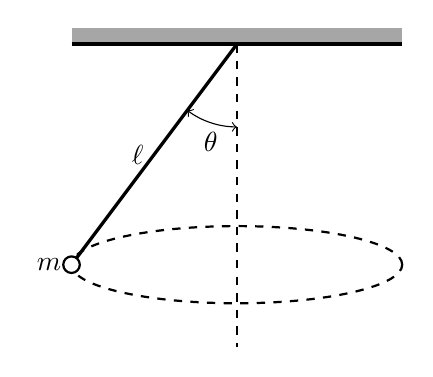
\begin{tikzpicture}[scale=.7]
          \draw[thick,dashed] ellipse (3 and .7);
          \draw[thick,dashed] (0,4)--(0,-1.5);
          \draw[very thick] (-3,0)--(0,4) node[midway,left]{$\ell$};
          \draw[thick,fill=white] (-3,0) circle (.15) node[left]{$m$};
          \draw[<->] (0,2.5) arc (270:270-atan(3/4):1.5)
          node[midway,below]{$\theta$};
          \fill[gray!70] (-3,4) rectangle (3,4.3);
          \draw[ultra thick] (-3,4)--(3,4);
        \end{tikzpicture}
      \end{center}
    }
    
    \question Which of the following diagrams best shows the forces acting on
    the ball as it moves in a circle?
    \label{conical1}

    \begin{oneparchoices}
      \choice
      \begin{tikzpicture}[vectors,scale=1.3]
        \fill circle (.05);
        \draw (0,0)--(0,-1) node[right]{$W$};
        \draw (0,0)--(1.3,0) node[right]{$F_c$};
        \draw[rotate=30] (0,0)--(1.5,0) node[right]{$T$};
      \end{tikzpicture}
      
      \choice
      \begin{tikzpicture}[vectors,scale=1.3]
        \fill circle (.05);
        \draw (0,0)--(0,-1) node[right]{$W$};
        \draw (0,0)--(1.5,0) node[right]{$T$};
      \end{tikzpicture}
      
      \choice
      \begin{tikzpicture}[vectors,scale=1.3]
        \fill circle (.05);
        \draw (0,0)--(0,-1) node[right]{$W$};
        \draw[rotate=30] (0,0)--(1.5,0) node[right]{$T$};
      \end{tikzpicture}

      \choice
      \begin{tikzpicture}[vectors,scale=1.3]
        \fill circle (.05);
        \draw (0,0)--(0,-1) node[right]{$W$};
        \draw (0,0)--(1.5,0) node[right]{$F_c$};
        \draw (0,0)--(0,1) node[right]{$T$};
      \end{tikzpicture}
      
      \choice
      \begin{tikzpicture}[vectors,scale=1.3]
        \fill circle (.05);
        \draw (0,0)--(0,-1) node[right]{$W$};
        \draw[rotate=120] (0,0)--(1.5,0) node[left]{$T$};
      \end{tikzpicture}
    \end{oneparchoices}
    \label{ball1}
    \columnbreak
    
    \question In terms of $m$, $\ell$ and $\theta$ and universal constants, the
    magnitude of the tension $T$ is
    \begin{choices}
      \choice $mg$
      \choice $mg\cos\theta$
      \choice $mg\sin\theta$
      \correctchoice $\dfrac{mg}{\cos\theta}$
      \choice $\dfrac{mg}{\sin\theta}$
    \end{choices}
    
    \question Which of the following expressions correct gives the speed at
    which the ball is travelling in terms of $\theta$, $\ell$ and universal
    constants?
    \label{conical2}
    \begin{choices}
      \choice $\sqrt{\ell g}$
      \choice $\sqrt{\ell g\sin\theta}$
      \choice $\sqrt{\ell g\cos\theta}$
      \choice $\sqrt{\ell g\tan\theta}$
      \choice $\sqrt{\ell g\sin\theta\tan\theta}$
    \end{choices}

%    \uplevel{
%      \centering
%      \begin{tikzpicture}[scale=1.3]
%        \begin{scope}[thick]
%          \draw[->] (0,0) arc (-90:0:1);
%          \draw (1,1) arc (0:90:1);
%          \draw[->] (0,2)--(-1,2);
%          \draw (0,2)--(-2,2);
%          \draw[->] (-2,2) arc (90:180:1);
%          \draw (-3,1) arc (180:280:1);
%          \draw[->] (-2,0)--(-1,0);
%          \draw(-2,0)--(0,0);
%          \fill ( 0,0) circle (.05) node[below]{$D$};
%          \fill ( 0,2) circle (.05) node[above]{$A$};
%          \fill (-2,2) circle (.05) node[above]{$B$};
%          \fill (-2,0) circle (.05) node[below]{$C$};
%          \fill (-2,1) circle (.05);
%          \fill ( 0,1) circle (.05);
%        \end{scope}
%      \end{tikzpicture}
%    }
%    \question A speed skater races around a track in which the sides are equal
%    length and parallel and the curves are semicircular. The skater keeps a
%    constant speed throughout one entire lap. She starts at point $A$ and
%    travels counterclockwise around the track for one lap. Which of the
%    following graphs best represents the magnitude of the skater's acceleration
%    as a function of time for one lap?
%    \begin{choices}
%      \choice
%      \begin{tikzpicture}
%        \draw[axes] (0,0)--(6.6,0) node[right]{$t$};
%        \draw[axes] (0,0)--(0,1.3) node[above]{$a$};
%        \draw[very thick] (0,0)--(1.5,0)--(1.5,1)--(3,1)--(3,0)--(4.5,0)
%        --(4.5,1)--(6,1)--(6,0);
%      \end{tikzpicture}
%
%      \choice
%      \begin{tikzpicture}
%        \draw[axes] (0,0)--(6.6,0) node[right]{$t$};
%        \draw[axes] (0,0)--(0,1.3) node[above]{$a$};
%        \draw[very thick] (0,0)--(1.5,0)--(3,1)--(4.5,1)--(6,0);
%      \end{tikzpicture}
%
%      \choice
%      \begin{tikzpicture}
%        \draw[axes] (0,0)--(6.6,0) node[right]{$t$};
%        \draw[axes] (0,0)--(0,1.3) node[above]{$a$};
%        \draw[very thick] (0,0)--(1.5,1)--(1.5,0)--(3,0)--(3,1)--(4.5,0)
%        --(6,0);    
%      \end{tikzpicture}
%
%      \choice
%      \begin{tikzpicture}
%        \draw[axes] (0,0)--(6.6,0) node[right]{$t$};
%        \draw[axes] (0,0)--(0,1.3) node[above]{$a$};
%        \draw[very thick] (0,0)--(1.5,0) to[out=0,in=240] (3,1)--(4.5,1)
%        to [out=-60,in=180] (6,0);
%      \end{tikzpicture}
%     
%      \choice
%      \begin{tikzpicture}
%        \draw[axes] (0,0)--(6.6,0) node[right]{$t$};
%        \draw[axes] (0,0)--(0,1.3) node[above]{$a$};
%        \draw[very thick] (0,0)--(1.5,1)--(3,1)--(3,0)--(4.5,0)--(6,1);
%      \end{tikzpicture}
%    \end{choices}
  \end{questions}
  \setcounter{lastmc}{\value{question}}
\end{multicols*}
\newpage

%\genfreetitle{6}{CIRCULAR MOTION}{3}
%\genfreedirections

\begin{questions}
  \setcounter{question}{\value{lastmc}}
  \question A mass $m$ attached to a string of length $2r$ swings, starting at
  rest when the string is horizontal, until the string is vertical. At the
  instant the string is vertical, the mass makes contact with the horizontal
  surface, the string is cut, and the mass continues along a frictionless track
  as shown below.
  \begin{center}
    \vspace{-.1in}
    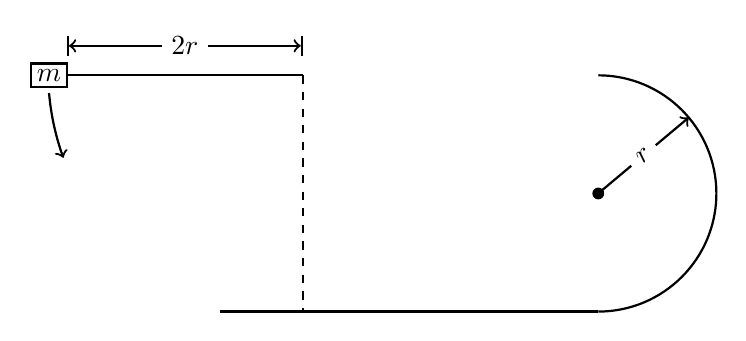
\begin{tikzpicture}[scale=1.5]
      \begin{scope}[thick]
        \draw (0,0)--(-2,0);
        \draw[|<->|] (0,.25)--(-2,.25) node[midway,fill=white]{$2r$};
        \draw (-2,.1) rectangle (-2.3,-.1) node[midway]{$m$};
        \draw[->] (-2.15,-.15) arc (185:200:2.15);
        \draw[dashed] (0,0)--(0,-2);
        \draw (-.7,-2)--(2.5,-2);
        \draw (2.5,-2) arc (-90:90:1);
        \fill (2.5,-1) circle (.05);
        \draw[rotate around={40:(2.5,-1)},->] (2.5,-1)--(3.5,-1)
        node[midway,fill=white,rotate=40]{$r$};
      \end{scope}
    \end{tikzpicture}
  \end{center}
  \begin{parts}
    \part What is the speed of the mass attached to the string the instant the
    string is cut?
    \vspace{\stretch1}
    
    \part Sketch the forces acting on the mass when it is in the position shown
    below.
    \begin{center}
      \begin{tikzpicture}[scale=2]
        \begin{scope}[thick]
          \draw (0,-2)--(2.5,-2);
          \draw (2.5,-2) arc (-90:90:1);
          \begin{scope}[rotate around={40:(2.5,-1)}]
            \draw[dashed] (2.5,-1)--(3.5,-1);
            \draw[fill=gray!50] (3.5,-.93) rectangle (3.36,-1.07);
          \end{scope}
          \draw[dashed] (2.5,-1)--(2.5,0);
          \draw (2.5,-.6) arc (90:40:.4) node[midway,above]{$\theta$};
        \end{scope}
      \end{tikzpicture}
    \end{center}
    \uplevel{
      When the mass is in the position shown above,
    }
    \part Find the object's speed as a function of $\theta$
    \vspace{\stretch1}
    
    \part Find the object's centripetal acceleration as a function of $\theta$
    \vspace{\stretch1}
    
    \part Determine at what angle $\theta$ the mass will fall of the track
    \vspace{\stretch1}
  \end{parts}
  \newpage

  % TAKEN FROM 2014 AP PHYSICS C MECHANICS EXAM FREE-RESPONSE QUESTION 2
  \uplevel{
    \cpic{.7}{ramp-circle}
  }
  \question A small block of mass $m$ starts from rest at the top of a
  frictionless ramp, which is at a height $h$ above a horizontal tabletop, as
  shown in the side view above. The block slides down the smooth ramp and
  reaches point $P$ with a speed $v_0$. After the block reaches point $P$
  at the bottom of the ramp, it slides on the tabletop guided by a circular
  vertical wall with radius $R$, as shown in the top view. The tabletop has
  negligible friction, and the coefficient of kinetic friction between the
  block and the circular wall is $\mu$.
  \begin{parts}
    \part Derive an expression for the height of the ramp $h$. Express your
    answer in terms of $v_0$, $m$, and fundamental constants, as
    appropriate.
    \vspace{\stretch1}
    
    \uplevel{
      A short time after passing point $P$, the block is in contact with
      the wall and moves with a speed of $v$.
    }
 
    \part Is the vertical component of the net force on the block upward,
    downward, or zero?
      
    \vspace{.1in}
    \underline{\hspace{.3in}} Upward\hspace{.2in}
    \underline{\hspace{.3in}} Downward\hspace{.2in}
    \underline{\hspace{.3in}} Zero
    
    \vspace{.1in}Justify your answer.
    \vspace{\stretch1}
    
    \part On the figure below, draw an arrow starting on the block to
    indicate the direction of the horizontal component of the net force on
    the moving block when it is at the position shown.
    \cpic{.3}{ramp-circle-top}
    \newpage
    
    \uplevel{
      Express your answers to the following in terms of $v_0$, $v$, $m$,
      $R$, $\mu$, and fundamental constants, as appropriate.
    }

    \part Determine an expression for the magnitude of the normal force $N$
    exerted on the block by the circular wall as a function of $v$.
    \vspace{\stretch1}
    
    \part Derive an expression for the magnitude of the tangential acceleration
    of the block at the instant the block has attained a speed of $v$.
    \vspace{\stretch1}
    
    \part Derive an expression for $v(t)$, the speed of the block as a
    function of time $t$ after passing point $P$ on the track.
    \vspace{\stretch2}
  \end{parts}
  \newpage

  % TAKEN FROM THE 2004 AP PHYSICS C MECHANICS EXAM FREE-RESPONSE QUESTION 1
  \uplevel{
    \cpic{.4}{swing}
  }
  \question A rope of length $L$ is attached to a support at point $C$. A person
  of mass $m_1$ sits on a ledge at position A holding the other end of the rope
  so that it is horizontal and taut, as shown above. The person then drops off
  the ledge and swings down on the rope toward position $B$ on a lower ledge
  where an object of mass $m_2$ is at rest. At position $B$ the person grabs
  hold of the object and simultaneously lets go of the rope. The person and
  object then land together in the lake at point $D$, which is a vertical
  distance $L$ below position $B$. Air resistance and the mass of the rope are
  negligible. Derive expressions for each of the following in terms of
  $m_1$, $m_2$, $L$, and fundamental constants.
  \begin{parts}
    \part The speed of the person just before the collision with the object
    \vspace{\stretch1}
    
    \part The tension in the rope just before the collision with the object
    \vspace{\stretch1}
    
    \part The speed of the person and object just after the collision
    \vspace{\stretch1}
    
    \part The ratio of the kinetic energy of the person-object system before
    the collision to the kinetic energy after the collision
    \vspace{\stretch1}
    \newpage
    
    \part The total horizontal displacement $x$ of the person from position
    $A$ until the person and object land in the water at point $D$.
    \vspace{\stretch1}
  \end{parts}
\end{questions}
\end{document}
